\documentclass[aspectratio=169,12pt]{beamer}
\usepackage[utf8]{inputenc}
\usepackage{amsmath, amssymb}
\usepackage{booktabs}
\usepackage{colortbl}
\usepackage{hyperref}
\usepackage{makecell}
\usepackage{ragged2e}
\usepackage{bytefield}
\usepackage{tikz}
\usetikzlibrary{arrows.meta, positioning, shapes.geometric, calc, tikzmark, shapes.misc}
\usetheme{Madrid}

\title{Computer Structure}
\subtitle{System}
\author{Lihu Rappoport}
\date{}

% Clock macro - draws a clock at given location
\newcommand{\drawclock}[1]{
    \begin{scope}[shift={(#1)}]
        \draw[thick] (0,0) circle (0.12);
        \draw[thick] (0,0) -- (0,0.08);
        \draw[thick] (0,0) -- (0.05,-0.03);
    \end{scope}
}

\begin{document}

\frame{\titlepage}


\begin{frame}{Basic DRAM chip}
\begin{itemize}
\item The DRAM memory is implemented as a 2-dimensional array of cells
\begin{itemize}
\item Arranged in rows and columns
\end{itemize}
\end{itemize}

\begin{center}
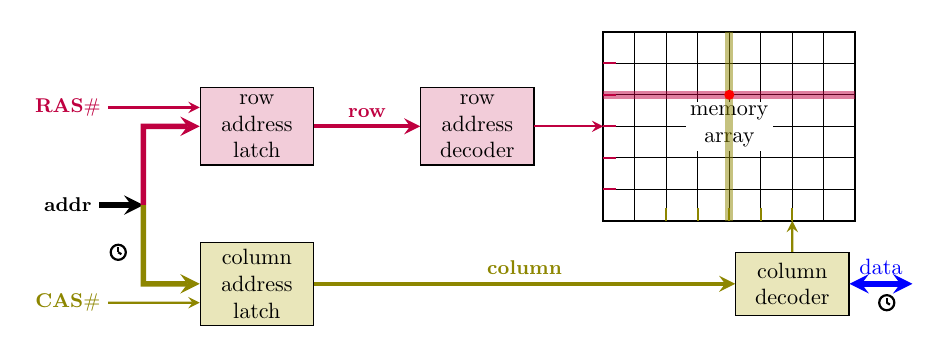
\begin{tikzpicture}[scale=0.8, transform shape,
    block/.style={draw, minimum width=1.8cm, minimum height=1cm, align=center},
    decoder/.style={draw, minimum width=1.8cm, minimum height=1.2cm, align=center},
    signal/.style={->, >=stealth, thick},
    label/.style={font=\small\bfseries}
]

% Row Address Latch
\node[block, text width=1.5cm, fill=purple!20] (rowlatch) at (0,0) {row address latch};

% Column Address Latch
\node[block, text width=1.5cm, fill=olive!20] (collatch) at (0,-2.5) {column address latch};

% Row Address decoder
\node[decoder, text width=1.5cm, fill=purple!20] (rowdecoder) at (3.5,0) {row address decoder};

% Column decoder
\node[block, text width=1.5cm, fill=olive!20] (coldecoder) at (8.5,-2.5) {column decoder};

% Memory array - draw as grid
\draw[thick] (5.5,1.5) rectangle (9.5,-1.5);
\foreach \x in {6,6.5,7,7.5,8,8.5,9} {
    \draw (\x,1.5) -- (\x,-1.5);
}
\foreach \y in {1,0.5,0,-0.5,-1} {
    \draw (5.5,\y) -- (9.5,\y);
}
\node[align=center, fill=white, inner sep=2pt] at (7.5,0) {memory\\array};

% Input signals
\node[label, purple] (ras) at (-3,0.3) {RAS$\#$};
\draw[signal, purple] (ras) -- (ras -| rowlatch.west);

\node[label, olive] (cas) at (-3,-2.8) {CAS$\#$};
\draw[signal, olive] (cas) -- (cas -| collatch.west);

\coordinate (addr_split) at (-1.8,-1.25);

\node[label] (addr) at (-3,-1.25) {addr};
\draw[signal, line width=2pt] (addr.east) -- (addr_split);
% Branch to row and column latches
\draw[signal, purple, line width=2pt] (addr_split) -- (-1.8,0) -- (rowlatch.west);
\draw[signal, olive, line width=2pt] (addr_split) -- (-1.8,-2.5) -- (collatch.west);

% Clock symbols next to latches
\drawclock{-2.2,-2}

% Connections between blocks
\draw[signal, purple, line width=1.5pt] (rowlatch.east) -- node[above, font=\small\bfseries, purple] {row} (rowdecoder.west);
\draw[signal, olive, line width=1.5pt] (collatch.east) -- node[above, font=\small\bfseries, olive] {column} (coldecoder.west);

% Row decoder to memory array with highlighted row
\draw[signal, purple] (rowdecoder.east) -- (5.5,0);
% Draw wordlines and highlight one
\foreach \y in {1,0.5,0,-0.5,-1} {
    \draw[purple, thick] (5.5,\y) -- (5.7,\y);
}
% Highlight one row
\draw[purple, line width=3pt, opacity=0.5] (5.5,0.5) -- (9.5,0.5);

% Column decoder to memory array with highlighted column
\draw[signal, olive] (coldecoder.north) -- (8.5,-1.5);
% Draw bitlines and highlight one
\foreach \x in {6.5,7,7.5,8,8.5} {
    \draw[olive, thick] (\x,-1.5) -- (\x,-1.3);
}
% Highlight one column
\draw[olive, line width=3pt, opacity=0.5] (7.5,1.5) -- (7.5,-1.5);

% Mark intersection
\fill[red] (7.5,0.5) circle (0.08);

% Data I/O - horizontal arrow
\draw[signal, blue, line width=2pt, <->] 
  (coldecoder.east) 
    -- node[midway, above, blue]{data} 
  ++(1,0);

% Clock symbol near data
\drawclock{10,-2.8}

\end{tikzpicture}
\end{center}

\vspace{-0.5cm}
\textbf{DRAM access sequence:}
\begin{enumerate}
\item Row address on bus → Assert RAS$\#$ to latch row
\item Column address on bus → Assert CAS$\#$ to latch column (after t$_{RCD}$ delay)
\item Data available after CAS latency (CL)
\end{enumerate}

\end{frame}
\end{document}